%----------------------------------------------------------------------------------------
%    PACKAGES AND THEMES
%----------------------------------------------------------------------------------------

\documentclass[aspectratio=169,xcolor=dvipsnames]{beamer}
\usetheme{SimpleDarkBlue}

\usepackage{hyperref}
\usepackage{graphicx} % Allows including images
\usepackage{booktabs} % Allows the use of \toprule, \midrule and \bottomrule in tables
\usepackage{caption} % Allows the usage of \captionsetup
\usepackage{enumitem}
\setlist[itemize,1]{label=\textbullet}
\setlist[itemize,2]{label=--}

\usepackage[T1]{fontenc}
\usepackage{cascadia-code}

%----------------------------------------------------------------------------------------
%    TITLE PAGE
%----------------------------------------------------------------------------------------

\title{Ateliers Créactifs Raspberry Pi}
\subtitle{Découverte de l'univers Raspberry Pi. Utilisation de cette carte électronique et exploration des possibilités.}

\author{Jean Bourgies, François Marelli, Ugo Proietti}

\date{10 février 2025}

%----------------------------------------------------------------------------------------
%    PRESENTATION SLIDES
%----------------------------------------------------------------------------------------

\begin{document}

\begin{frame}
    % Print the title page as the first slide
    \titlepage
\end{frame}

\begin{frame}{Table des matières}
    % Throughout your presentation, if you choose to use \section{} and \subsection{} commands, these will automatically be printed on this slide as an overview of your presentation
    \tableofcontents
\end{frame}

%------------------------------------------------
\section{Découverte de la carte Raspberry Pi}
%------------------------------------------------

\begin{frame}{Raspberry Pi}
    \begin{columns}[c] % 'c' ensures vertical centering for both columns

        \column{.4\textwidth} % Left column
        \begin{figure}
            
\includegraphics[width=1\textwidth]{images/logo-rpi.png}
        \end{figure}

        \column{.6\textwidth} % Right column
        \begin{itemize}
            \item Carte de développement
            \item Créée en 2012 à des fins pédagogiques
            \item Libre de droit
            \item Modèles différents
        \end{itemize}

    \end{columns}
\end{frame}

%------------------------------------------------

\begin{frame}{Série Raspberry Pi}
    \begin{columns}[c] % 'c' ensures vertical centering for both columns

        \column{1\textwidth} % Left column
        \begin{figure}
            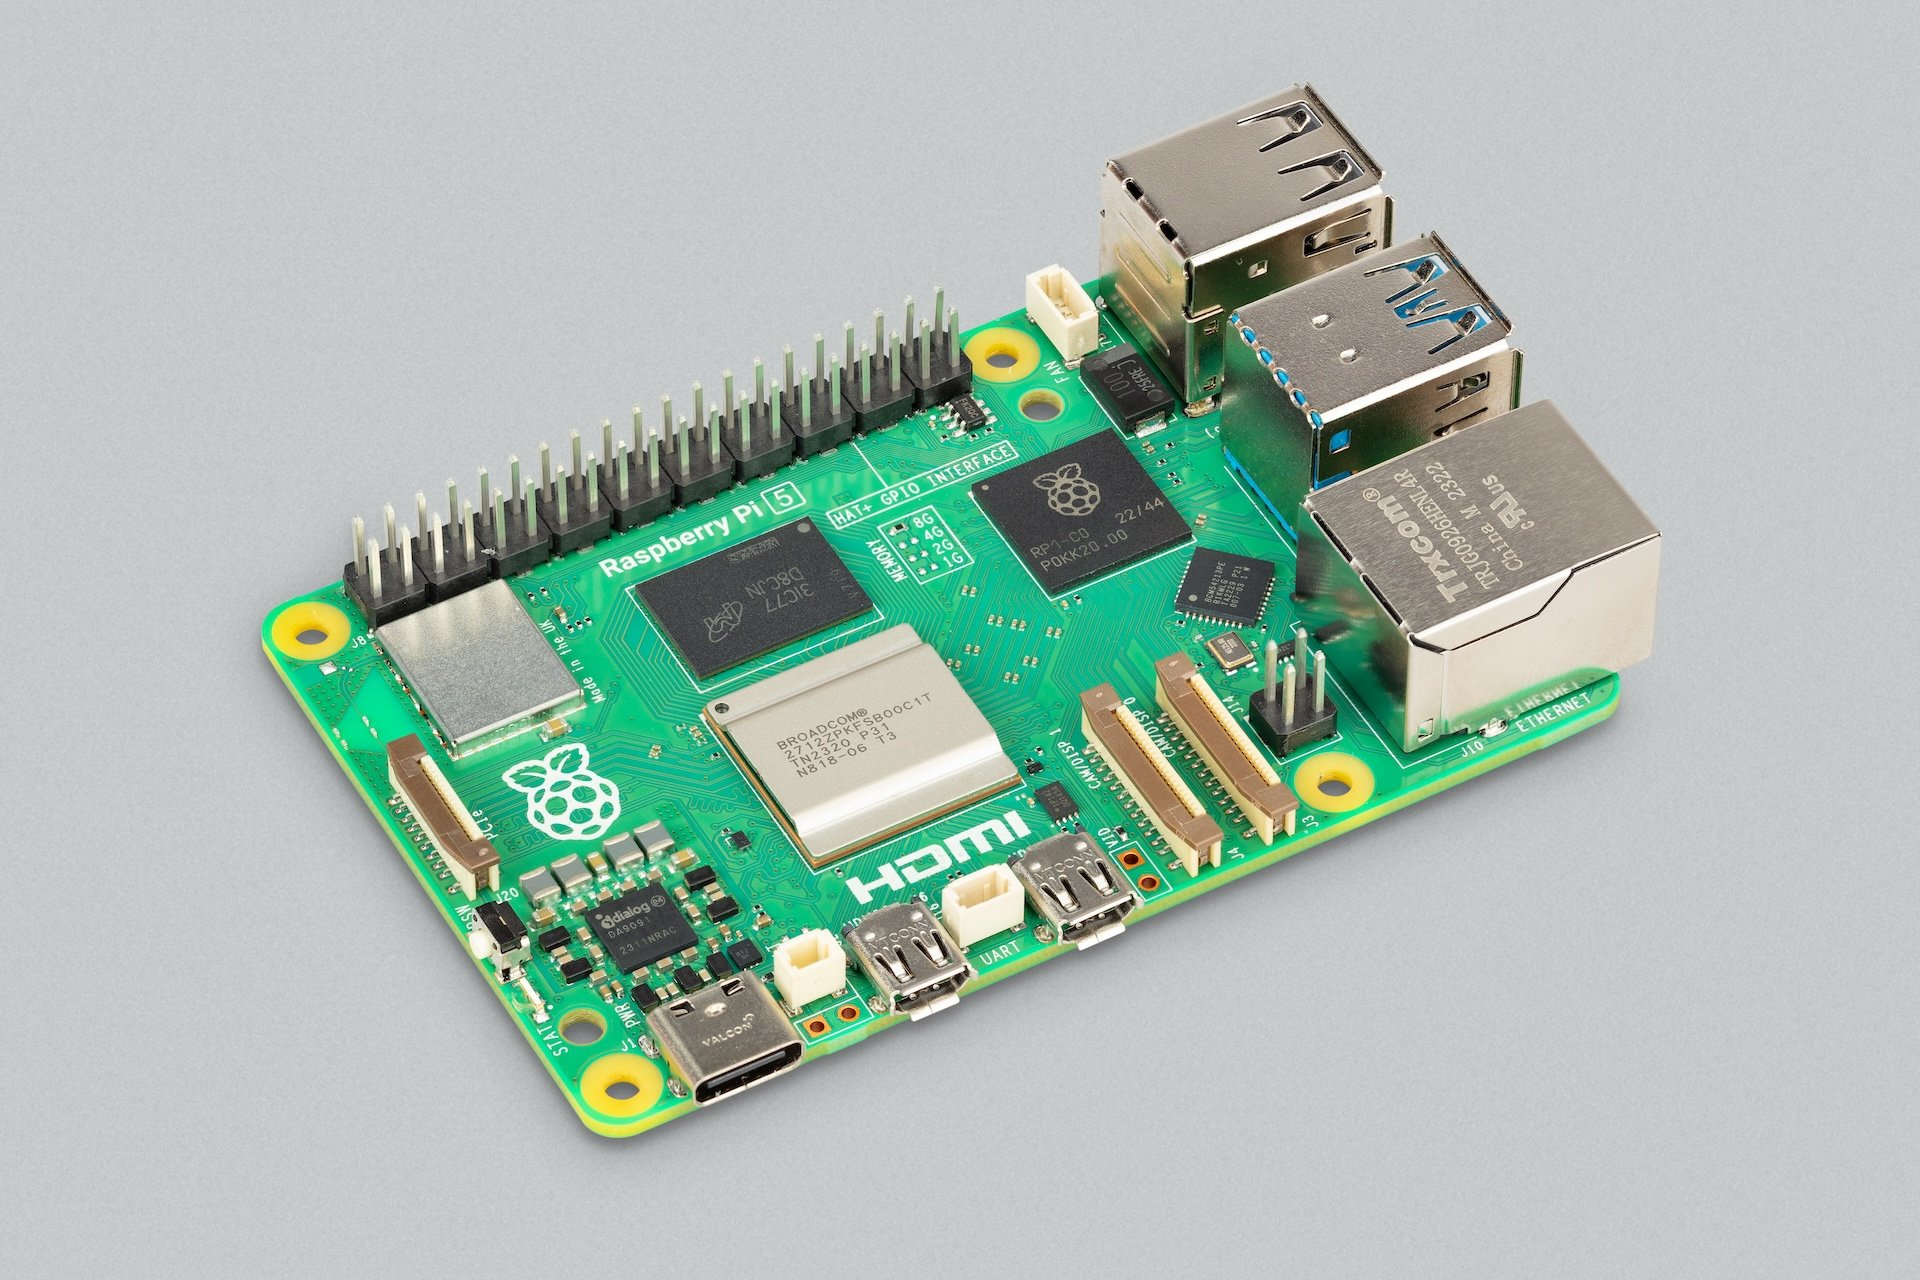
\includegraphics[width=1\textheight]{images/rpi-5.jpg}
            \captionsetup{labelformat=empty}
            \caption{Raspberry Pi 5}
        \end{figure}

    \end{columns}
\end{frame}

%------------------------------------------------

\begin{frame}{Série Clavier}
    \begin{columns}[c] % 'c' ensures vertical centering for both columns

        \column{1\textwidth} % Left column
        \begin{figure}
            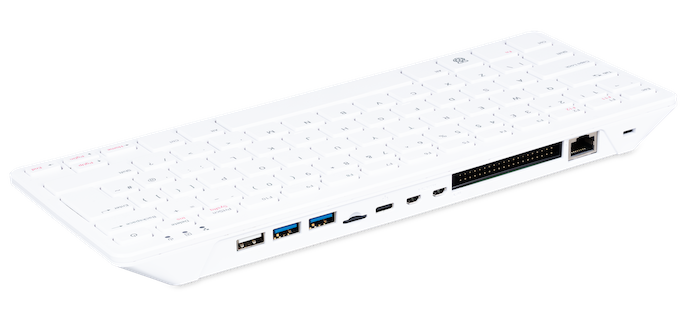
\includegraphics[width=1\textheight]{images/rpi-500.png}
            \captionsetup{labelformat=empty}
            \caption{Raspberry Pi 500}
        \end{figure}

    \end{columns}
\end{frame}

%------------------------------------------------

\begin{frame}{Série Zero et Pico}
    \begin{columns}[c] % 'c' ensures vertical centering for both columns

        \column{0.5\textwidth} % Left column
        \begin{figure}
            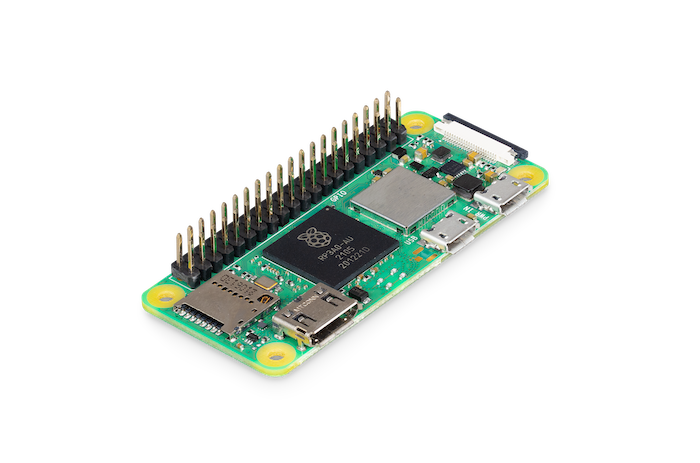
\includegraphics[width=1\textwidth]{images/rpi-zero.png}
            \captionsetup{labelformat=empty}
            \caption{Raspberry Pi Zero 2 WH}
        \end{figure}

        \column{0.5\textwidth} % Left column
        \begin{figure}
            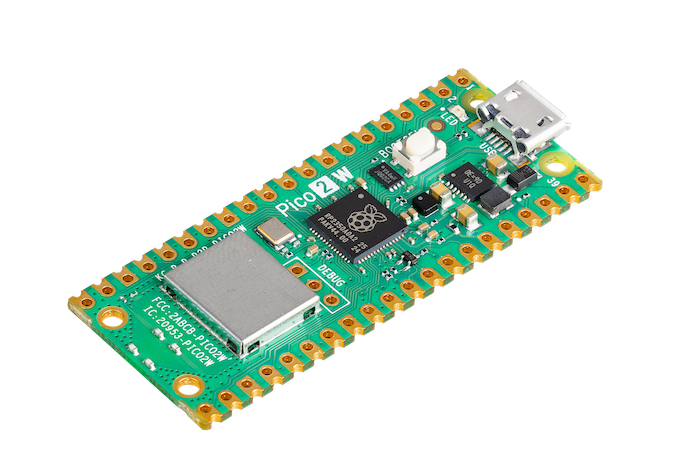
\includegraphics[width=1\textwidth]{images/rpi-pico.png}
            \captionsetup{labelformat=empty}
            \caption{Raspberry Pi Pico 2 W}
        \end{figure}

    \end{columns}
\end{frame}

%------------------------------------------------
\section{Découverte du système d'exploitation}
%------------------------------------------------

\begin{frame}{Raspberry Pi OS}
    \begin{columns}[c] % 'c' ensures vertical centering for both columns

        \column{.4\textwidth} % Left column
        \begin{figure}
            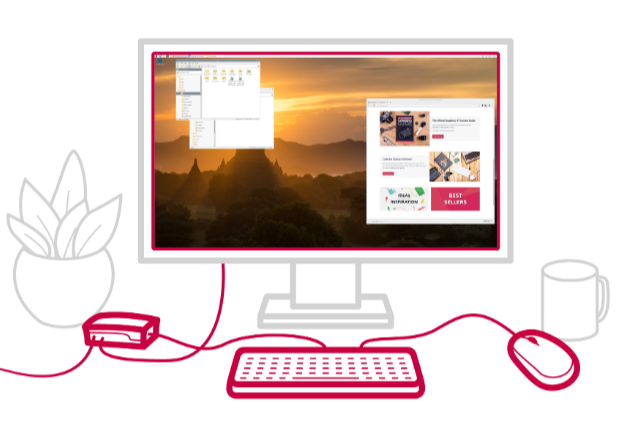
\includegraphics[width=1\textwidth]{images/rpi-os.png}
        \end{figure}

        \column{.6\textwidth} % Right column
        \begin{itemize}
            \item Système d'exploitation
            \item Basé sur Linux
            \item Spécialement conçu pour les cartes Raspberry Pi
        \end{itemize}

    \end{columns}
\end{frame}

%------------------------------------------------

\begin{frame}{Raspberry Pi Imager}
    \begin{columns}[c] % 'c' ensures vertical centering for both columns

        \column{.6\textwidth} % Left column
        \begin{figure}
            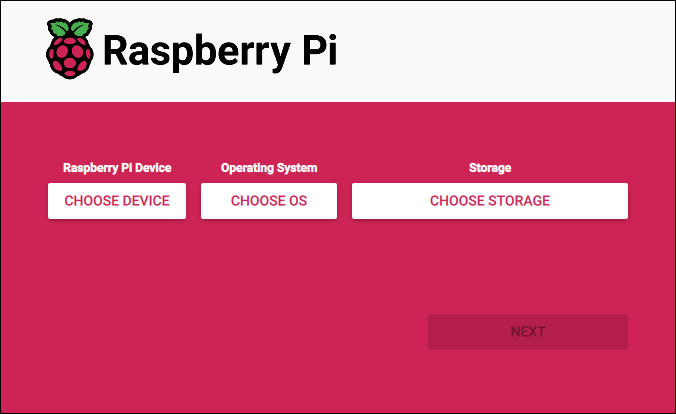
\includegraphics[width=1\textwidth]{images/rpi-imager-0.png}
        \end{figure}

        \column{.4\textwidth} % Right column
        \begin{itemize}
            \item Outil d'installation
            \item Conçu pour Raspberry Pi
            \item Compatible avec tous les systèmes d'exploitation
        \end{itemize}

    \end{columns}
\end{frame}

%------------------------------------------------

\begin{frame}{Raspberry Pi Imager}
    \begin{columns}[c] % 'c' ensures vertical centering for both columns

        \column{.6\textwidth} % Left column
        \begin{figure}
            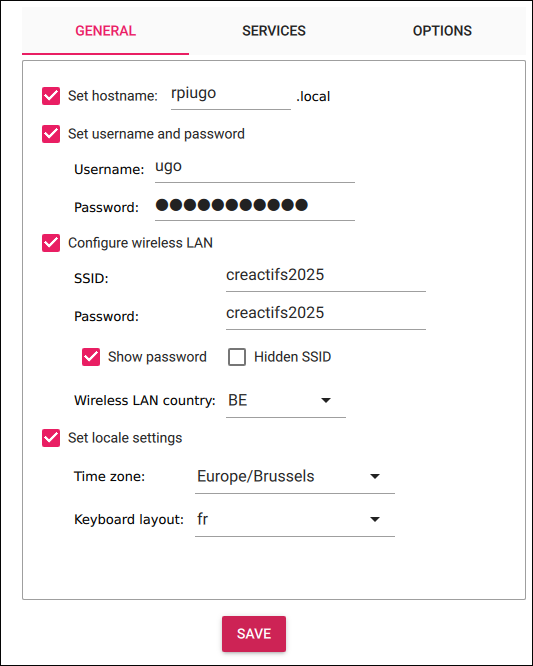
\includegraphics[width=0.6\textwidth]{images/rpi-imager-1.png}
        \end{figure}

        \column{.4\textwidth} % Right column
        \begin{itemize}
            \item Menu de paramétrage
            \item Accessible avec CTRL + SHIFT + X
        \end{itemize}

    \end{columns}
\end{frame}

%------------------------------------------------

\begin{frame}{Raspberry Pi Imager}
    \begin{columns}[c] % 'c' ensures vertical centering for both columns

        \column{.6\textwidth} % Left column
        \begin{figure}
            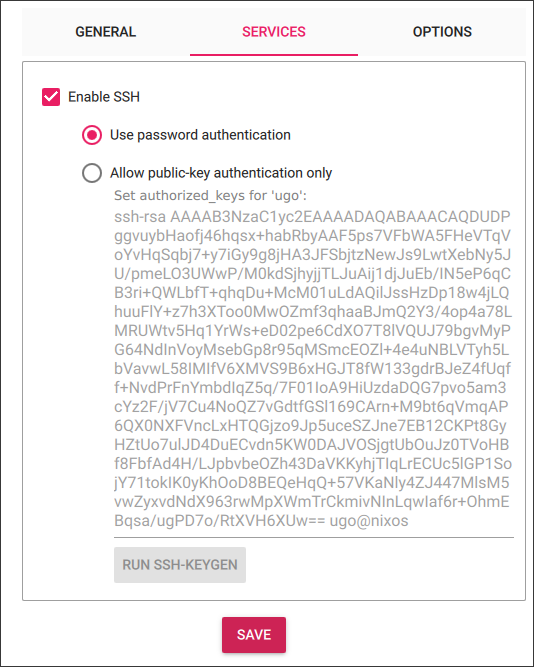
\includegraphics[width=0.6\textwidth]{images/rpi-imager-2.png}
        \end{figure}

        \column{.4\textwidth} % Right column
        \begin{itemize}
            \item Menu de paramétrage
            \item Accessible avec CTRL + SHIFT + X
        \end{itemize}

    \end{columns}
\end{frame}

%------------------------------------------------

\begin{frame}{Raspberry Pi Imager}
    \begin{columns}[c] % 'c' ensures vertical centering for both columns

        \column{.6\textwidth} % Left column
        \begin{figure}
            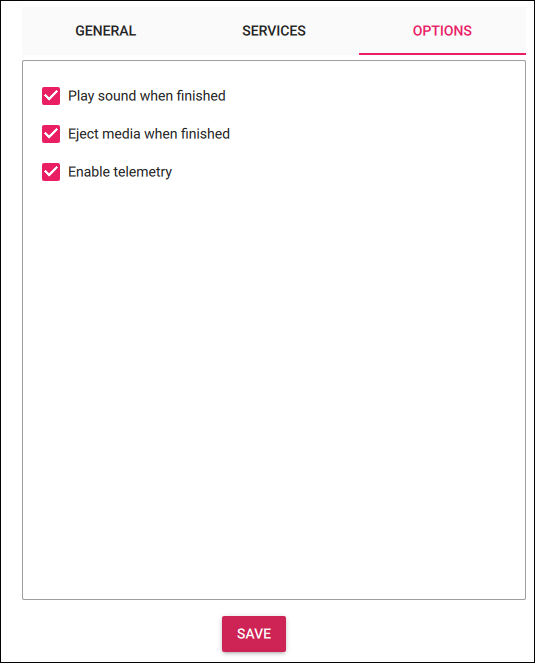
\includegraphics[width=0.6\textwidth]{images/rpi-imager-3.png}
        \end{figure}

        \column{.4\textwidth} % Right column
        \begin{itemize}
            \item Menu de paramétrage
            \item Accessible avec CTRL + SHIFT + X
        \end{itemize}

    \end{columns}
\end{frame}

%------------------------------------------------

\begin{frame}{Linux}
    \begin{columns}[c] % 'c' ensures vertical centering for both columns

        \column{.6\textwidth} % Left column
        \begin{figure}
            
\includegraphics[width=0.4\textwidth]{images/tux.png}
            \captionsetup{labelformat=empty}
            \caption{Tux, la mascotte de Linux}
        \end{figure}

        \column{.6\textwidth} % Right column
        \begin{itemize}
            \item Performances
            \item Personnalisation
            \item Sécurité
        \end{itemize}

    \end{columns}
\end{frame}

%------------------------------------------------

\begin{frame}{Questions}
    \begin{center}
        Questions / Remarques / Réflexions
    \end{center}
\end{frame}

%------------------------------------------------
\section{Première utilisation}
%------------------------------------------------

\begin{frame}{Bienvenue}
    \begin{columns}[c] % 'c' ensures vertical centering for both columns

        \column{0.75\textwidth} % Left column
        \begin{figure}
            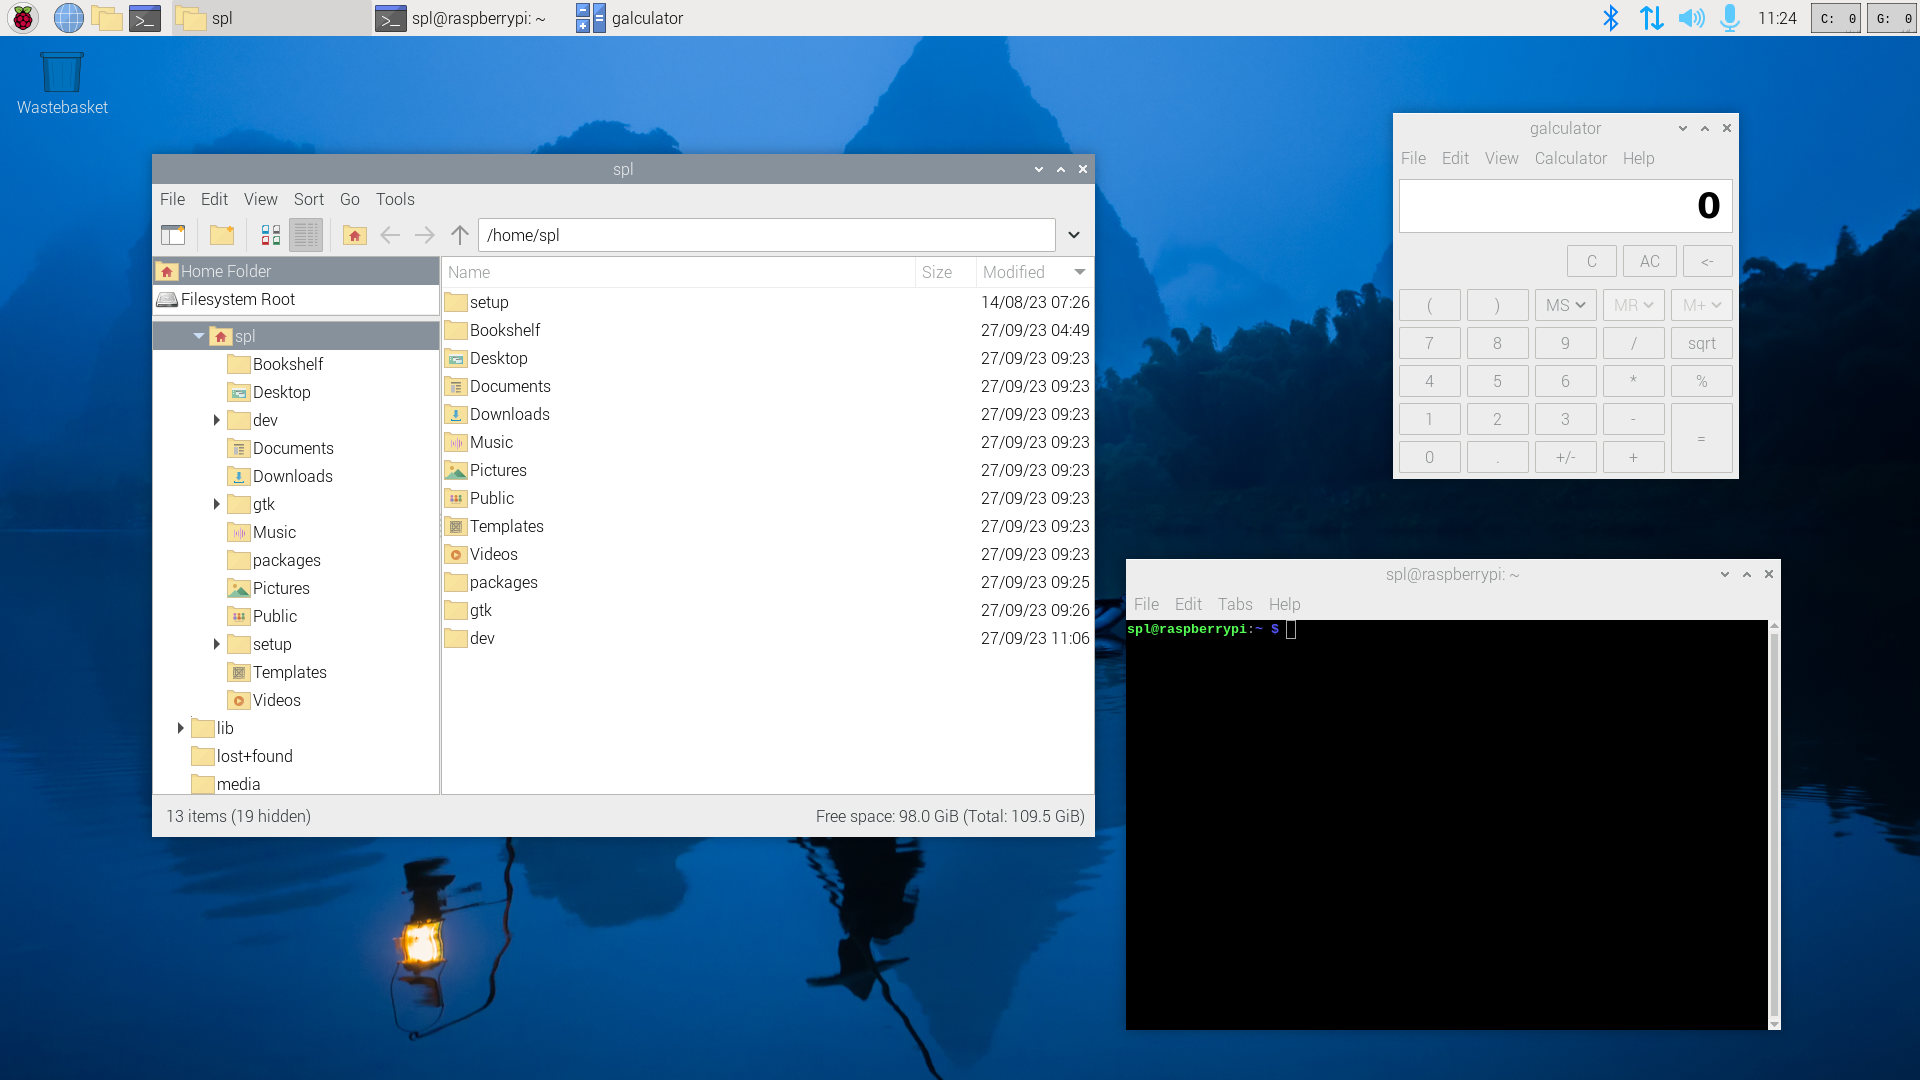
\includegraphics[width=1\textwidth]{images/rpi-os-welcome.png}
        \end{figure}

        \column{0.25\textwidth} % Right column
        \begin{center}
            Terminal
            \begin{figure}
                
\includegraphics[width=0.7\textwidth]{images/terminal.png}
            \end{figure}

            Fichiers
            \begin{figure}
                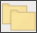
\includegraphics[width=0.7\textwidth]{images/fichiers.png}
            \end{figure}
        \end{center}

    \end{columns}
\end{frame}

%------------------------------------------------

\begin{frame}{Commandes de base du terminal 1/3}

    Navigation dans les fichiers/dossiers
    \begin{itemize}
        \item \texttt{ls} : liste les fichiers/dossiers
        \item \texttt{cd [chemin]} : change le dossier courant
        \item \texttt{pwd} : afficher le chemin actuel
    \end{itemize}

    Gestion des fichiers/dossiers
    \begin{itemize}
        \item \texttt{touch [nom]} : créer un fichier vide
        \item \texttt{mkdir [nom]} : crée un dossier vide
        \item \texttt{rm [nom]} : supprime un fichier/dossier
        \item \texttt{cp [source] [destination]} : copie un fichier/dossier
        \item \texttt{mv [source] [destination]} : déplace ou renomme un fichier/dossier
        \item \texttt{nano [fichier]} : change le contenu d'un fichier
    \end{itemize}

\end{frame}

%------------------------------------------------

\begin{frame}{Commandes de base du terminal 2/3}

    Informations système
    \begin{itemize}
        \item \texttt{whoami} : affiche votre nom d'utilisateur
        \item \texttt{df -h} : montre l'espace disque disponible
        \item \texttt{top} : surveille les processus en temps réel
    \end{itemize}

    Gestion des droits
    \begin{itemize}
        \item \texttt{chmod [mode] [fichier/dossier]} : change les permissions
        \item \texttt{chown [utilisateur] [fichier/dossier]} : change le propriétaire
    \end{itemize}

    Recherche
    \begin{itemize}
        \item \texttt{find [chemin] -name [nom]} : cherche un fichier/dossier par nom
        \item \texttt{grep [mot] [fichier]} : cherche un mot-clé dans un fichier
    \end{itemize}

\end{frame}

%------------------------------------------------

\begin{frame}{Commandes de base du terminal 3/3}

    Gestion des logiciels
    \begin{itemize}
        \item \texttt{sudo apt update} : mise à jour de la liste des programmes disponibles
        \item \texttt{sudo apt upgrade} : mise à jour des programmes
        \item \texttt{sudo apt install [nom]} : installe un programme
    \end{itemize}

    Gestion de la carte RPI
    \begin{itemize}
        \item \texttt{sudo raspi-config} : ouverture de l'outil de configuration
    \end{itemize}

\end{frame}

%------------------------------------------------

\begin{frame}{Exercices}

    \begin{block}{Écriture dans un fichier}
        Dans le dossier \texttt{\textasciitilde/Documents}, créez un fichier nommé \texttt{groupe} dans lequel vous indiquerez les prénoms des membres de votre groupe.
    \end{block}

    \begin{block}{Recherche de l'espace disque libre}
        Dans le dossier \texttt{\textasciitilde/Documents}, créez un fichier nommé \texttt{disque} dans lequel vous indiquerez le pourcentage d'espace disque utilisé.
    \end{block}

    \begin{block}{Mise à jour du système et installation d'un programme}
        Mettre à jour son système, installer le programme \texttt{cowsay} et exécuter la commande \texttt{cowsay "Bienvenue aux ateliers Raspberry Pi!"}
    \end{block}

\end{frame}

\end{document}
